\chapter[Materials and Methods]{Materials and Methods}
\label{Materials}

In this chapter, we present in the first two sections the methodologies of both methods we used to solve the LMDD problem. Further, we present the hybrid method, that unifies both approaches.

\section[Mathematical Model]{Mathematical Model}
\label{Mathematical_Model}

We propose a Mixed-Integer Linear Programming (MILP) model to solve the problem. First, in Section~\ref{graph-modeling}, we illustrate in detail how to construct a graph representing the spatio-temporal permits shared by the drones.

\subsection{Graph Modeling} \label{graph-modeling}

Following the flow network problem paradigm, we model our spatio-temporal permits as a directed graph (digraph) $G = (V, A)$, where:

\begin{itemize}
  \item $V$ is the set of nodes representing the airspace and virtual drone locations.
  \item $A$ is the set of directed arcs representing the permitted transitions between nodes.
\end{itemize}

The temporal component is omitted here as we are primarily interested in representing the problem's spatial topology.

\begin{figure}[H]
  \centering
  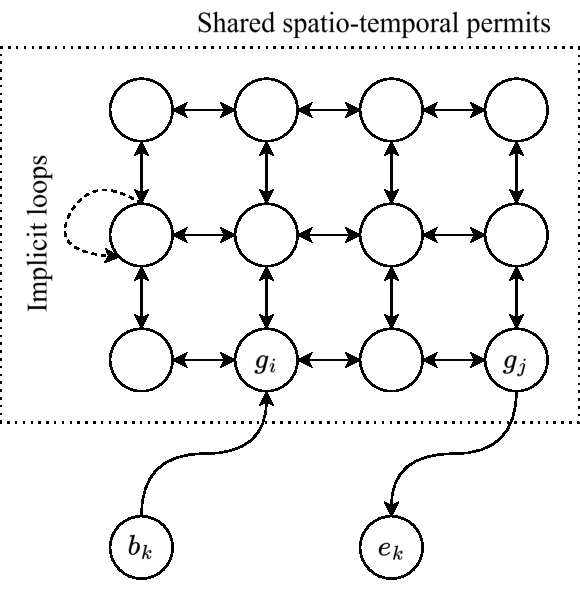
\includegraphics[width=0.8\textwidth]{img/graph_model.pdf}
  \caption[graph modelling]{Graph modelling. Source: The authors.}
  \label{fig:graph_model}
\end{figure}



Figure~\ref{fig_graph} depicts a simplified 2D grid-shaped example of a shared airspace (without altitude) for illustrative purposes. The dotted rectangular area represents the physical 2D airspace.

\subsubsection{Virtual Nodes for Drones}

In addition to the shared airspace, we introduce two virtual nodes for each drone $k$:

\begin{itemize}
  \item A source node $b_k$: This represents the starting point of drone $k$'s mission.
  \item A sink node $e_k$: This represents the ending point of drone $k$'s mission.
\end{itemize}


Each drone $k$ must initiate its mission at $b_k$ and conclude it at $e_k$. These virtual nodes streamline the model by circumventing the need to explicitly handle individual drone start and end positions.

Here's a breakdown of the virtual node connections:

\begin{itemize}
  \item Drone $k$ can only remain in $b_k$ or exit it to the shared airspace.
  \item Once exited, no drone (including $k$ itself) can re-enter $b_k$.
  \item A priori, any drone $k$ can enter its designated sink node $e_k$. However, constraints will be formulated in the mathematical programming section to ensure only drone $k$ enters its corresponding $e_k$.
\end{itemize}

\subsubsection{Drone Loitering}

Since we're dealing with rotary-wing vehicles, the model allows drones to remain (loiter) at a node for a certain time. To accommodate this, we include a loop arc for every node in the graph, encompassing both physical and virtual source/sink nodes. For clarity, these loops are implicitly considered in the example of Figure~\ref{fig_graph} and not explicitly depicted.

Including loops simplifies the mathematical programming model by avoiding the need to address potential exceptions.

\subsection{Parameters}

Below are listed the parameters that are constants of the problem:

\begin{itemize}
\item $T$: maximum time allowed for the mission (limits drone movement);
\item $b_k$: initial virtual vertex representing the initial position (begin) of drone $k$;
\item $e_k$: final virtual vertex representing the final position (end) of drone $k$;
\item $\mathcal{R}$: set of drones;
\item $\mathcal{G}$: digraph $(\mathcal{V}, \mathcal{A})$ representing the airspace;
\item $\mathcal{V}$: set of vertices of $\mathcal{G}$ representing each cell of the airspace or virtual vertex;
\item $\mathcal{B} \subset \mathcal{V}$: set of initial virtual vertices $b_k$;
\item $\mathcal{E} \subset \mathcal{V}$: set of final virtual vertices $e_k$;
\item $\mathcal{S}$: set $\mathcal{V} \setminus (\mathcal{B} \cup \mathcal{E})$ of vertices exclusively representing the shared airspace, i.e., eliminating virtual vertices;
\item $\mathcal{A}$: set of arcs $(i,j) \in \mathcal{A}$ of $\mathcal{G}$ connecting airspace cells to each other or a virtual vertex to the airspace.
\end{itemize}

\subsection{Indices}

In the equations, we use the following iteration indices:

\begin{itemize}
\item $k$ : drone $\implies$ $k \in \mathcal{R}$;
\item $t$ : time $\implies$ $1 \leq t \leq T $;
\item $i,j,l$ : vertices $\implies$ $i, j, l \in \mathcal{V}$.
\end{itemize}

\subsection{Decision Variables}

Below are listed the decision variables of the model:

\begin{itemize}
\item $x_{i,j,t}^k = 1 \iff$ drone $k$ jumps from $i$ to $j$ at time $t$.
\end{itemize}


\subsection{Objective Function}

We choose an objective function that minimizes the total sum of the number of drone movements,
\begin{equation}\label{eq:fobj}
\min
\sum_{k \in \mathcal{R}}
\sum_{t=1}^T
\sum_{ \; (i,j) \in \mathcal{A}:\ j \notin (\mathcal{E} \cup \mathcal{B})} x_{i,j,t}^{k}\text{,}
\end{equation}
counting $n-1$ jumps for each drone that performs $n$ jumps, since the jump to the final virtual vertex cannot be counted as a vertex with cost for the drone mission. Loops at initial virtual vertices are also disregarded.

\subsection{Constraints}

The set of constraints are described in the following.

\subsubsection{Movement Start}

We require that each drone starts its mission, \begin{equation}\label{eq:restr_inicio}
\sum_{t=1}^{T}
\sum_{j \in \mathcal{S}}
x_{b_k,j,t}^k = 1, \quad \forall k \in \mathcal{R}
\end{equation},  by jumping from its virtual initial node $b_k$ to the shared airspace.

\subsubsection{Flow Conservation}

 The flow conservation is also addressed,  \begin{equation}\label{eq:restr_fluxo}
\sum_{j \in \mathcal{V}} x_{i,j,t-1}^{k} =
\sum_{l \in \mathcal{V}} x_{j,l,t}^{k}, \quad
\forall j \in \mathcal{V}, \forall k \in \mathcal{R}, \forall t \in \{2, \ldots, T\} \; \text{,}
\end{equation} ensuring the consistency of allowed movements defined by the graph $\mathcal{G}$

\subsubsection{Border Condition}

Initially, under the border condition at time $t=0$, we consider there is a loop flow of drones at the virtual initial vertices.
This flow is redirected into the problem by the flow conservation constraint. \begin{equation}\label{eq:restr_borda}
    x_{i,j,0}^k = \left\{
    \begin{matrix}
        1, & \text{if}\ i=b_k \land j=b_k,\\
        0, & \text{otherwise}.
    \end{matrix}
    \right.
    \quad \forall k \in \mathcal{R}, \forall (i,j) \in A  \; \text{.}
\end{equation} For all other variables at time $t=0$, we consider a flow equal to zero.

\subsubsection{Mutual exclusion of vertex occupation}

We ensure that no drones occupy the same position,

\begin{equation}\label{eq:restr_ocupacao}
\sum_{k \in \mathcal{R}}
\sum_{j \in \mathcal{V}}
x_{i,j,t}^{k} \leq 1, \quad \forall j \in \mathcal{V}, \forall t \in \{1, \ldots, T\} \; \text{,}
\end{equation} that is, each vertex $j \in \mathcal{V}$ is occupied by at most one drone.

\subsubsection{Mission Accomplishment}

Every drone $k$ needs to complete its mission, 

\begin{equation}\label{eq:restr_fim}
\sum_{t=1}^{T}
\sum_{i \in \mathcal{S}}
x_{i,e_k,t}^k \geq 1, \quad \forall k \in \mathcal{R} \; \text{,}
\end{equation} i.e., reaching its final virtual vertex $e_k$ is required.


\section[Heuristic]{Heuristic}
\label{Heuristic}

In this section, we present our heuristic approach for tackling the problem, focusing on the utilization of a distance measure as a heuristic metric to organize drones in ascending order(prioritized planning) based on their start and end points. This prioritized order is then employed in an iterative Breadth-First Search (BFS) on the temporal graph. The BFS process dynamically updates the constraints of occupied positions(conflict-based search), creating a sequential refinement of the temporal graph with each newly generated minimum path. By combining heuristic sorting and iterative BFS, our approach aims to efficiently navigate the solution space, providing a balance between effective path planning and adaptability to evolving constraints in the context of drone delivery.


MAPF algorithms are recognized for their versatility with various distance metrics \cite{Weise2023}. In our specific scenario, we chose the Euclidean Distance as our metric of choice. This decision stems from its efficacy as a tiebreaker for drones that traverse the same number of cells in the minimum path, as observed with the Manhattan Distance. Notably, drones may share the same Manhattan Distance but diverge in Euclidean Distance, particularly when paths involve changes in direction. For instance, drones following a straight-line trajectory in the minimum path encounter fewer potential movement positions, while paths with changes in axis may introduce additional possibilities, making Euclidean Distance a valuable discriminant in such cases. This strategic use of the Euclidean Distance enhances the overall performance and adaptability of our algorithm in navigating complex drone delivery scenarios, as exemplified in \ref{ssec:example}, especially in scenarios with high traffic congestion where having more possibilities is crucial for finding local optimal solutions.

While conflict-based search has exponential complexity \cite{DBLP:conf/socs/GordonFS21}, our algorithm has polynomial complexity in function of size of the grid and number of drones. However, we cannot guarantee optimality, and this is expected since, even in the 2D grid case, MAPF where each agent has three or more possible directions of movement is also NP-hard\cite{geft2023finegrained}.


\begin{table}[H]
  \centering
  \caption{Notation used in the Algorithm.}
  \label{tab:notation}
  \begin{tabular}{ll}
    \toprule
    Notation & Definition \\
    \midrule
    $\mathcal{V}$ &Set of vertices in the graph $: (i,j,t)$ \\
    $\mathcal{E}$ & Set of edges  \\
    $\mathcal{D}$ & Set of drones \\
    $\mathcal{S}$ & Set of already scheduled vertices \\
    $\mathcal{P}_d \subseteq \mathcal{V} $ & Path of drone $d$ \\
    $\mathcal{G} = (\mathcal{V},\mathcal{E}) $ & Temporal Graph \\
    \bottomrule
  \end{tabular}
\end{table}

Formally, using the notation in Table \ref{tab:notation}, we can create a temporal graph $\mathcal{G}$ that naturally represents our problem. Since the set of vertex $\mathcal{V}:= (i,j,t)$ represents every possible position $(i,j)$ at any given time $t$ in our problem.  This modeling approach streamlines the search for optimal solutions in an efficient manner. The representation allows us to capture the possibility of a drone waiting at its position at a specific time $t_{wait}$ through the graph edges. We achieve this by defining the set of outgoing edges for a vertex $v^*=(i^*,j^*,t^*$ as $\mathcal{E}_{v^*} = \{ (i^*+1,j^*,t^*+1), (i^*,j^*+1,t^*+1), (i^*-1,j^*,t^*+1), (i^*,j^* -1,t^*+1), (i^*,j^*,t^*+1) \}$. The edge $(i^*,j^*,t^*+1)$ means that the drone chooses a path in which it decides to wait a time step. We define our algorithm sequentially as follows:

\begin{enumerate}

   \item \textbf{Drones Sorting}: We begin by ascending sorting the drones using the Euclidean Distance as a heuristic, given by \( \sqrt{(x_{\text{begin}} - x_{\text{end}})^2 + (y_{\text{begin}} - y_{\text{end}})^2} \), \begin{equation}
        \mathcal{D}_{\text{sorted}} = \text{sort}(\mathcal{D}, \text{heuristic}) \; \text{.}
    \end{equation}
    
\item \textbf{Path for Each Drone}: For each drone \(d\) in the sorted order, we compute the path \(P_d\) using Breadth-First Search (BFS) on the graph \(\mathcal{G}\). The BFS is performed with the constraints imposed by the set \(\mathcal{S}\), \begin{equation}
        \forall d \in \mathcal{D}_{\text{sorted}}: \quad \mathcal{P}_d = \text{BFS}(\mathcal{G}, d) \; \text{.}
    \end{equation}
    
    \item \textbf{Constraints Update}: After determining paths for the respective drone, we update the set of already scheduled vertices \(\mathcal{S}\) immediately following the execution of each BFS sequentially. This update involves incorporating the vertices covered by the path into the existing set of constraints (previously scheduled paths), \begin{equation}
        \mathcal{S} = \mathcal{S} \cup \bigcup_{d \in \mathcal{D}_{\text{sorted}}} \mathcal{P}_d \; \text{.}
    \end{equation}

   Indeed, the \textbf{constraints} ensure that no two drones occupy the same vertex at the same time, \begin{equation}
    \forall d, d' \in \mathcal{D}, d \neq d', \forall (i, j, t) \in \mathcal{P}_d, (i, j, t) \notin \mathcal{P}_{d'} \; \text{.}
\end{equation}

    
\end{enumerate}

In the computational aspect, our implementation follows the standard implementation of BFS in 3D grids, since the time $t$ can be simply thought as a third dimension. The main difference of common implementations is the addition of a \textit{map}, that is a Red Black Tree, to manage the set of scheduled positions. This addition adds $\mathcal{O}(\log n)$ in the complexity of our algorithm. The pseudo algorithm of the heuristic is described in Algorithm \ref{alg:grid-bfs}.


\begin{algorithm}[H]
    \label{alg:grid-bfs}
    \DontPrintSemicolon
    \KwData{Grid dimensions $N$ (rows) and $M$ (columns), Number of drones $K$, List of drones \textit{drones}}
    \KwResult{Paths for each drone considering constraints}

    \BlankLine
    \ForEach{\textit{drone} in \textit{drones}}{
        Initialize data structures for BFS: \textit{bfs\_queue}, \textit{parent}, \textit{visited}\;
        Set \textit{flight\_time} of \textit{drone} to -1\;
        \While{No valid path found for \textit{drone}}{
            Increment \textit{flight\_time} of \textit{drone}\;
            Enqueue \textit{drone\_begin} with \textit{flight\_time} into \textit{bfs\_queue}\;
            \While{\textit{bfs\_queue} is not empty}{
                Dequeue a position and time \;
                \If{Position is the destination of \textit{drone}}{
                    Reconstruct and schedule path for \textit{drone}\;
                    \Return path\;
                }
                \If{Position is scheduled}{
                \textit{\textbf{Continue}}
                    \;
                }
                \For{Neighbor positions}{
                    \If{Position is valid and not visited}{
                        \If{Position is scheduled and no schedule discovered in neighbors yet}{
                            
                            Enqueue current position and \textit{flight\_time + 1} \;
                            
                            \textit{\textbf{Continue}} \;
                        }
                        Mark position as visited\;
                        Store parent information\;
                        Enqueue the neighbor position into \textit{bfs\_queue}\;
                    }
                }
            }
        }
    }
    \caption{Path Planning for Drones using BFS}
\end{algorithm}


\subsection{Example} \label{ssec:example}

\begin{figure}[h]
    \centering
    \begin{tikzpicture}[scale=.8, every node/.style={minimum size=1cm}]

        % Define quadcopter style
        \tikzset{
            quadcopter/.style={
                quadcopter side,
                fill=white,
                draw=gray,
                minimum width=1cm,
                below=of second-scope, 
            },
        }
        
        % Add another drone
        \node (quadcopterGreen) [quadcopter side, fill=white, draw=greenMW, minimum width=1cm, rotate=0] at (5,1) {};

        \node (quadcopterBrown) [quadcopter side, fill=white, draw=brown, minimum width=1cm, rotate=0] at (5,-11.3) {};

        \node (quadcopterOrange) [quadcopter side, fill=white, draw=orange, minimum width=1cm, rotate=0] at (4.4,-14.3) {};

        \node (quadcopterBlue) [quadcopter side, fill=white, draw=blue, minimum width=1cm, rotate=0] at (-5,-8.2) {};
        
        % Último Escopo (t=6)
        \begin{scope}[yshift=-423, every node/.append style={yslant=0.5, xslant=-1}, yslant=0.5, xslant=-1]

            

            \fill[white, fill opacity=0.9] (0,0) rectangle (5,5);
            
            \draw[step=4mm, black] (0,0) grid (5,5);
            \draw[black, thick] (0,0) rectangle (5,5); % Borders
            \fill[orange] (2.05,2.05) rectangle (2.35,2.35); % center pixel
            \node (centerBegint2) at (2.2,2.2) {B}; % place 'B' in the center
            % \fill[greenMW] (1.65,2.05) rectangle (1.95,2.35); % left
            % \fill[greenMW] (2.45,2.05) rectangle (2.75,2.35); % right
            \fill[orange] (2.05,1.95) rectangle (2.35,1.65); % bottom
            \fill[orange,yshift=-11.2] (2.05,1.95) rectangle (2.35,1.65); % bottom
            \fill[orange,yshift=-22.5] (2.05,1.95) rectangle (2.35,1.65); % bottom
            \fill[orange,yshift=-33.5] (2.05,1.95) rectangle (2.35,1.65); % bottom
            
            %\fill[greenMW] (2.05,2.45) rectangle (2.35,2.75); % top
            % 8 -pixel setting
           
            % \fill[greenMW] (2.75,1.95) rectangle (2.45,1.65); % bottom-right
            % \fill[greenMW] (1.65,1.95) rectangle (1.95,1.65); % bottom-left
            
            \node (landedOrange) at (1.5,0.8) {};

            \node(pathdestinyt6) [black, font=\bfseries] at ([yshift=-45.3]centerBegint2) {E};
        \end{scope}



        % Penúltimo Escopo (t=5)
        \begin{scope}[yshift=-340, every node/.append style={yslant=0.5, xslant=-1}, yslant=0.5, xslant=-1]
            \fill[white, fill] (0,0) rectangle (5,5);
            \draw[step=4mm, black] (0,0) grid (5,5);
            \draw[black, thick] (0,0) rectangle (5,5); % Borders
            \fill[orange!55] (2.05,2.05) rectangle (2.35,2.35); % center pixel
            \node (centerBegint3) at (2.2,2.2) {B}; % place 'B' in the center

            \fill[orange!55,xshift=-22.6] (2.45,2.05) rectangle (2.75,2.35); % most left
            

            \node (landedBrown) at (1.5,0.6) {};

            %\fill[blue] (1.65,2.05) rectangle (1.95,2.35); % left
            % left X
            \draw[orange] (1.65,2.05) -- (1.95,2.35);
            \draw[orange] (1.65,2.35) -- (1.95,2.05);
            % left bottom X
            \draw[orange, yshift=-11.3] (1.65,2.05) -- (1.95,2.35);
            \draw[orange, yshift=-11.3] (1.65,2.35) -- (1.95,2.05);   
            % most left X
            \draw[orange, xshift=-11.3] (1.65,2.05) -- (1.95,2.35);
            \draw[orange, xshift= -11.3] (1.65,2.35) -- (1.95,2.05);   

            \fill[orange!55,xshift=11.3] (2.45,2.05) rectangle (2.75,2.35); % most right
            % most right X
            \draw[orange, xshift=34.4] (1.65,2.05) -- (1.95,2.35);
            \draw[orange, xshift=34.4] (1.65,2.35) -- (1.95,2.05);

            % bottom center right X
            \draw[orange, xshift=34.4, yshift= -11.3] (1.65,2.05) -- (1.95,2.35);
            \draw[orange, xshift=34.4, yshift= -11.3] (1.65,2.35) -- (1.95,2.05);

            %  top center right X
            \draw[orange, xshift=34.4, yshift= 11.3] (1.65,2.05) -- (1.95,2.35);
            \draw[orange, xshift=34.4, yshift= 11.3] (1.65,2.35) -- (1.95,2.05);
            
            % most most right X
            \draw[orange, xshift=34.4 + 11.3] (1.65,2.05) -- (1.95,2.35);
            \draw[orange, xshift=34.4 + 11.3] (1.65,2.35) -- (1.95,2.05);

            

            \fill[orange!55] (2.45,2.05) rectangle (2.75,2.35); % right
            
            \fill[orange!55] (2.05,2.45) rectangle (2.35,2.75); % top
            \fill[orange!55, xshift=11.3] (2.05,2.45) rectangle (2.35,2.75); % top right
            \fill[orange!55, xshift=-11.3] (2.05,2.45) rectangle (2.35,2.75); % top left
            \fill[orange!55, yshift=11.3] (2.05,2.45) rectangle (2.35,2.75); % most top
            \fill[orange!55] (2.05,1.95) rectangle (2.35,1.65); % bottom

            \fill[orange!55, xshift= 11.3] (2.05,1.95) rectangle (2.35,1.65); % bottom right

            \fill[orange!55,yshift=-11.3] (2.05,1.95) rectangle (2.35,1.65); % most bottom
            
            %\fill[greenMW] (1.65,2.45) rectangle (1.95,2.75); % top-left 
            % top left X
            \draw[orange] (1.65,2.75) -- (1.95,2.45);
            \draw[orange] (1.65,2.45) -- (1.95,2.75);
            
            % top most left X
            \draw[orange, xshift=-11.3] (1.65,2.75) -- (1.95,2.45);
            \draw[orange, xshift=-11.3] (1.65,2.45) -- (1.95,2.75);
            
            % \draw[orange,xshift=-11.3] (1.65,2.75) -- (1.95,2.45);
            % \draw[orange,xshift=-11.3] (1.65,2.45) -- (1.95,2.75);   

            %\fill[greenMW] (2.45,2.45) rectangle (2.75,2.75); % top-right
            \draw[orange] (2.45,2.45) -- (2.75,2.75);
            \draw[orange] (2.45,2.75) -- (2.75,2.45);

            %\fill[greenMW] (2.75,1.95) rectangle (2.45,1.65); % bottom-right
            \draw[orange] (2.45,1.95) -- (2.75,1.65);
            \draw[orange] (2.45,1.65) -- (2.75,1.95);

            % top most X 
            \draw[orange,xshift= -34 +45.4,yshift=11] (1.65,2.75) -- (1.95,2.45);
            \draw[orange,xshift=-34 +45.4,yshift=11] (1.65,2.45) -- (1.95,2.75);

            % top most right X 
            \draw[orange,xshift= -34 +45.4 + 11.2,yshift=11] (1.65,2.75) -- (1.95,2.45);
            \draw[orange,xshift=-34 +45.4 + 11.2,yshift=11] (1.65,2.45) -- (1.95,2.75);

            % top most left X 
            \draw[orange,xshift= -34 +45.4 - 11.2,yshift=11] (1.65,2.75) -- (1.95,2.45);
            \draw[orange,xshift=-34 +45.4 - 11.2,yshift=11] (1.65,2.45) -- (1.95,2.75);

            % top most last X 
            \draw[orange,xshift= -34 +45.4 ,yshift=22.2] (1.65,2.75) -- (1.95,2.45);
            \draw[orange,xshift=-34 +45.4 ,yshift=22.2] (1.65,2.45) -- (1.95,2.75);

            % bottom most X
            \draw[orange,xshift= -34 +45.4,yshift=-34.4] (1.65,2.75) -- (1.95,2.45);
            \draw[orange,xshift=-34 +45.4,yshift=-34.4] (1.65,2.45) -- (1.95,2.75);

            % bottom most right X
            \draw[orange,xshift= -34 +45.4 +11.2 ,yshift=-34.4] (1.65,2.75) -- (1.95,2.45);
            \draw[orange,xshift=-34 +45.4 + 11.2,yshift=-34.4] (1.65,2.45) -- (1.95,2.75);

            % bottom most left X
            \draw[orange,xshift= -34 +45.4 -11.2 ,yshift=-34.4] (1.65,2.75) -- (1.95,2.45);
            \draw[orange,xshift=-34 +45.4  -11.2,yshift=-34.4] (1.65,2.45) -- (1.95,2.75);

            % bottom most last X
            \draw[orange,xshift= -34 +45.4,yshift=-45.8] (1.65,2.75) -- (1.95,2.45);
            \draw[orange,xshift=-34 +45.4,yshift=-45.8] (1.65,2.45) -- (1.95,2.75);

                    

            %\fill[blue] (1.65,1.95) rectangle (1.95,1.65); % bottom-left
            % 2. ring
            %\fill[greenMW] (1.25,1.55) rectangle (1.55,1.25); % bottom-left
            %\fill[greenMW] (0.85,1.55) rectangle (1.15,1.25); % bottom-left
            %\fill[greenMW] (0.85,1.15) rectangle (1.15,0.85); % bottom-left

            \fill[brown, xshift=22.7, yshift=-11.2] (1.25,0.75) rectangle (1.55,0.45); % bottom-left

            \node(pathdestinyt3) [black, font=\bfseries] at ([yshift=-45.3]centerBegint3) {E};
        \end{scope}


        % Escopo (t=4)
        \begin{scope}[yshift=-250, every node/.append style={yslant=0.5, xslant=-1}, yslant=0.5, xslant=-1]
            \fill[white, fill] (0,0) rectangle (5,5);
            \draw[step=4mm, black] (0,0) grid (5,5);
            \draw[black, thick] (0,0) rectangle (5,5); % Borders
            \fill[orange!55] (2.05,2.05) rectangle (2.35,2.35); % center pixel
            \node (centerBegint3) at (2.2,2.2) {B}; % place 'B' in the center
            
            %\fill[blue] (1.65,2.05) rectangle (1.95,2.35); % left
            \draw[orange] (1.65,2.05) -- (1.95,2.35);
            \draw[orange] (1.65,2.35) -- (1.95,2.05);   

            \node (landedBlue) at (1.1,2.3) {};

            % most right X
            \draw[orange, xshift=34.4] (1.65,2.05) -- (1.95,2.35);
            \draw[orange, xshift=34.4] (1.65,2.35) -- (1.95,2.05);  

            \fill[orange!55] (2.45,2.05) rectangle (2.75,2.35); % right
            \fill[orange!55] (2.05,2.45) rectangle (2.35,2.75); % top
            \fill[orange!55] (2.05,1.95) rectangle (2.35,1.65); % bottom
            
            %\fill[greenMW] (1.65,2.45) rectangle (1.95,2.75); % top-left
            \draw[orange] (1.65,2.75) -- (1.95,2.45);
            \draw[orange] (1.65,2.45) -- (1.95,2.75);   
            
            % \draw[orange,xshift=-11.3] (1.65,2.75) -- (1.95,2.45);
            % \draw[orange,xshift=-11.3] (1.65,2.45) -- (1.95,2.75);   

            %\fill[greenMW] (2.45,2.45) rectangle (2.75,2.75); % top-right
            \draw[orange] (2.45,2.45) -- (2.75,2.75);
            \draw[orange] (2.45,2.75) -- (2.75,2.45);

            %\fill[greenMW] (2.75,1.95) rectangle (2.45,1.65); % bottom-right
            \draw[orange] (2.45,1.95) -- (2.75,1.65);
            \draw[orange] (2.45,1.65) -- (2.75,1.95);

            % top most X 
            \draw[orange,xshift= -34 +45.4,yshift=11] (1.65,2.75) -- (1.95,2.45);
            \draw[orange,xshift=-34 +45.4,yshift=11] (1.65,2.45) -- (1.95,2.75);

            % bottom most X
            \draw[orange,xshift= -34 +45.4,yshift=-34.4] (1.65,2.75) -- (1.95,2.45);
            \draw[orange,xshift=-34 +45.4,yshift=-34.4] (1.65,2.45) -- (1.95,2.75);

            \fill[blue] (1.65,1.95) rectangle (1.95,1.65); % bottom-left
            % 2. ring
            %\fill[greenMW] (1.25,1.55) rectangle (1.55,1.25); % bottom-left
            %\fill[greenMW] (0.85,1.55) rectangle (1.15,1.25); % bottom-left
            %\fill[greenMW] (0.85,1.15) rectangle (1.15,0.85); % bottom-left

            \fill[brown, xshift=22.6] (1.25,0.75) rectangle (1.55,0.45); % bottom-left

            \node(pathdestinyt3) [black, font=\bfseries] at ([yshift=-45.3]centerBegint3) {E};
        \end{scope}

        % Terceiro Escopo (t=3)
        \begin{scope}[yshift=-166, every node/.append style={yslant=0.5, xslant=-1}, yslant=0.5, xslant=-1]
            \fill[white, fill opacity=0.9] (0,0) rectangle (5,5);
            \draw[step=4mm, black] (0,0) grid (5,5);
            \draw[black, thick] (0,0) rectangle (5,5); % Borders
            \fill[orange!55] (2.05,2.05) rectangle (2.35,2.35); % lighter orange for center pixel
            \node (centerBegint3) at (2.2,2.2) {B}; % place 'B' in the center
            \fill[blue] (1.65,2.05) rectangle (1.95,2.35); % left
            \draw[orange] (2.45,2.05) -- (2.75,2.35);
            \draw[orange] (2.45,2.35) -- (2.75,2.05);
            %\fill[greenMW] (2.05,2.45) rectangle (2.35,2.75); % top
            \draw[orange] (2.05,2.45) -- (2.35,2.75);
            \draw[orange] (2.05,2.75) -- (2.35,2.45);

            %\fill[greenMW] (2.05,1.95) rectangle (2.35,1.65); % bottom
            \draw[orange] (2.05,1.95) -- (2.35,1.65);
            \draw[orange] (2.05,1.65) -- (2.35,1.95);

            
            %\fill[greenMW] (1.65,2.45) rectangle (1.95,2.75); % top-left
            %\fill[greenMW] (2.45,2.45) rectangle (2.75,2.75); % top-right
            %\fill[greenMW] (2.75,1.95) rectangle (2.45,1.65); % bottom-right
            %\fill[greenMW] (1.65,1.95) rectangle (1.95,1.65); % bottom-left
            % 2. ring
            %\fill[greenMW] (1.25,1.55) rectangle (1.55,1.25); % bottom-left
            %\fill[greenMW] (0.85,1.55) rectangle (1.15,1.25); % bottom-left
            %\fill[greenMW] (0.85,1.15) rectangle (1.15,0.85); % bottom-left

            \fill[brown, xshift=11.3] (1.25,0.75) rectangle (1.55,0.45); % bottom-left

            \node(pathdestinyt3) [black, font=\bfseries] at ([yshift=-45.3]centerBegint3) {E};

            \node(midpointX) at (2.6, 2.2){};
            
        \end{scope}

        % Escopo do meio (t=2)
        \begin{scope}[yshift=-83, every node/.append style={yslant=0.5, xslant=-1}, yslant=0.5, xslant=-1]

            \node [quadcopter side,fill=white,draw=orange,minimum width=1cm,rotate=10] (quadcoptert2) at (1,7) {};

            \fill[white, fill opacity=0.9] (0,0) rectangle (5,5);

            \node (arrivalOrange) at (1.8,2.1) {};
            
            \draw[step=4mm, black] (0,0) grid (5,5);
            \draw[black, thick] (0,0) rectangle (5,5); % Borders
            \fill[orange] (2.05,2.05) rectangle (2.35,2.35); % center pixel
            \node (centerBegint2) at (2.2,2.2) {B}; % place 'B' in the center
            % \fill[greenMW] (1.65,2.05) rectangle (1.95,2.35); % left
            % \fill[greenMW] (2.45,2.05) rectangle (2.75,2.35); % right
            \fill[greenMW] (2.05,1.95) rectangle (2.35,1.65); % bottom
            \node (landedGreen) at (1.8,1.9) {};
            %\fill[greenMW] (2.05,2.45) rectangle (2.35,2.75); % top
            % 8 -pixel setting
            \fill[blue] (1.65,2.45) rectangle (1.95,2.75); % top-left
            % \fill[greenMW] (2.45,2.45) rectangle (2.75,2.75); % top-right
            % \fill[greenMW] (2.75,1.95) rectangle (2.45,1.65); % bottom-right
            % \fill[greenMW] (1.65,1.95) rectangle (1.95,1.65); % bottom-left
            % 2. ring
            % \fill[greenMW] (1.25,1.55) rectangle (1.55,1.25); % bottom-left
            % \fill[greenMW] (0.85,1.55) rectangle (1.15,1.25); % bottom-left
            % \fill[greenMW] (0.85,1.15) rectangle (1.15,0.85); % bottom-left
            \fill[brown] (1.25,0.75) rectangle (1.55,0.45); % bottom-left
            \node(pathdestinyt2) [black, font=\bfseries] at ([yshift=-45.3]centerBegint2) {E};
        \end{scope}

        % Primeiro Escopo (t=1)
        \begin{scope}[yshift=0, every node/.append style={yslant=0.5, xslant=-1}, yslant=0.5, xslant=-1]

           \node [quadcopter side,fill=white,draw=orange,minimum width=1cm,rotate=10] (quadcoptert1) at (3,7.6) {};
            
           \node (orangeTakeOff) at (2.5,1.8) {};
        
            \fill[white, fill opacity=0.9] (0,0) rectangle (5,5);
            \draw[step=4mm, black] (0,0) grid (5,5); % Grid definition
            \draw[black, thick] (0,0) rectangle (5,5); % Borders
            \fill[greenMW] (2.05,2.05) rectangle (2.35,2.35); % center pixel
            \draw[red, thin] (2.05,2.05) rectangle (2.35,2.35); % border
            \node (centerBegint1) at (2.2,2.2) {B}; % place 'B' in the center
            \fill[blue] (2.05,2.45) rectangle (2.35,2.75); % top
            % \fill[blue] (1.65,2.45) rectangle (1.95,2.75); % top-left
            % \fill[blue] (2.45,2.45) rectangle (2.75,2.75); % top-right
            % \fill[blue] (2.75,1.95) rectangle (2.45,1.65); % bottom-right
            % \fill[blue] (1.65,1.95) rectangle (1.95,1.65); % bottom-left
            % % 2. ring
            % \fill[blue] (1.25,1.55) rectangle (1.55,1.25); % bottom-left
            % \fill[blue] (0.85,1.55) rectangle (1.15,1.25); % bottom-left
            % \fill[blue] (0.85,1.15) rectangle (1.15,0.85); % bottom-left
            % \fill[blue] (1.25,0.75) rectangle (1.55,0.45); % bottom-left

            \fill[brown, xshift= -11.3] (1.25,0.75) rectangle (1.55,0.45); % bottom-left
            
            % Insert 'E' three squares down the center
            \node(pathdestinyt1) [black, font=\bfseries] at ([yshift=-45.3]centerBegint1) {E};
            
        \end{scope}

        % Draw annotations
        \draw[-latex, thick, gray, dashed] (-5.4,-3.5) node[left] {occupied} to[out=0, in=200] (-0.5,-4.1);

        \draw[-latex, thick, red] (quadcoptert1) to[out=35, in=90] node[midway, above] {failed takeoff} (orangeTakeOff);

        \draw[-latex, thick, orange] (quadcoptert2) to[out=0, in=10] node[very near start, above] {arrival} (arrivalOrange);

        %\draw[-latex, thick, orange] ([xshift=-10]centerBegint3) to[out=0, in=10] (midpointX);

        \draw[thick, green!60!black, dashed] (landedGreen) to[out=0, in=10] node[above, pos=0.45 , font=\footnotesize] {landed} (quadcopterGreen);

        \draw[thick, brown!, dashed] (landedBrown) to[out=0, in=10] node[ above, pos=1 , font=\footnotesize] {landed} (quadcopterBrown);

        \draw[thick, orange!, dashed] (landedOrange) to[out=0, in=10] node[ above, pos=0.75 , font=\footnotesize] {path found} (quadcopterOrange);

        \draw[thick, blue!60!white, dashed] (landedBlue) to[out=0, in=13] node[ above, pos=0.85 , font=\footnotesize] {landed} (quadcopterBlue);

        % Annotations
        \draw[thick, gray!60!black] (6,4) node {t=1};
        \draw[thick, gray!60!black] (6,0) node {t=2};
        \draw[thick, gray!60!black] (6,-3) node {t=3};
        \draw[thick, gray!60!black] (6,-6) node {t=4};
        \draw[thick, gray!60!black] (6,-9) node {t=5};
        \draw[thick, gray!60!black] (6.2,-12.4) node {t=6};
    \end{tikzpicture}
    \caption{Algorithm visualization. Source: The authors.}
    \label{fig:visualgo}
\end{figure}


In Figure \ref{fig:visualgo}, the algorithm visualization shows its ability to address corner cases, including take-off in occupied positions and collision avoidance.

The depicted scenario involves determining the route for the orange drone within a grid where blue, brown, and green drones have already established their scheduled routes. These pre-existing paths serve as constraints in the optimization problem.

Upon closer inspection of Figure \ref{fig:visualgo}, it is evident that both the orange and brown drones cover an equal number of positions in the grid. However, an important factor influencing the algorithm's decision-making is a heuristic chosen for prioritization. In this case, the heuristic involves considering the shorter Euclidean distance covered by the brown drone. Consequently, during the sorting process, the algorithm prioritizes the brown drone based on this chosen heuristic, irrespective of the equality in the number of positions traversed.



\subsection{Complexity Analysis and Boundedness}
\label{secc:complexity_analysis}

Given $K$ the number of drones and
$N, M$ the grid sizes, the number of rows, and the number of columns, respectively. We can analyze our algorithm regarding these inputs using asymptotic computational complexity.

The complexity of our algorithm is the worst case of a BFS in the temporal graph, considering the $\mathcal{O}(\log S)$ from the scheduled structure, where $S= N M T$ is the size of the search space. It can be seen that this would be $\mathcal{O}(N M T)\mathcal{O}(\log N M T)$, where $T$ is the maximum time a drone lands. However, $T$ is surely bounded by $\mathcal{O}(K N M)$. In addition, it can be shown that $T$ is bounded by $\mathcal{O}((N+M) K)$. An intuitive view of this is shown in \ref{fig:worst_path}, where we have three drones on a $3\times 4$ grid with the same initial position($s_i$) and final position($g_i$), where $i=1\dots3$. In this case, the shorter path for each drone is $n+m$,$n=3;m=4$, and in the worst case, we will wait for each drone to complete its path, thus $k(n+m)$ is an upper bound for our heuristic since our heuristic always chooses a shorter path than $k(n+m)$ because we do not wait for each drone to complete the path.   Then the complexity is bounded by $$\mathcal{O}((N+M) K N M \log((N+M) K N M))= \mathcal{O}(\max{(N,M)} N M K  \log(\max{(N,M)} N M K)) $$  $\approx \mathcal{O}(N^3  K \log(N^3 K) = \mathcal{O}(N^3  K \max{(\log N , \log K))} $, if the grid is square. 



\begin{figure}[H]
    \centering
    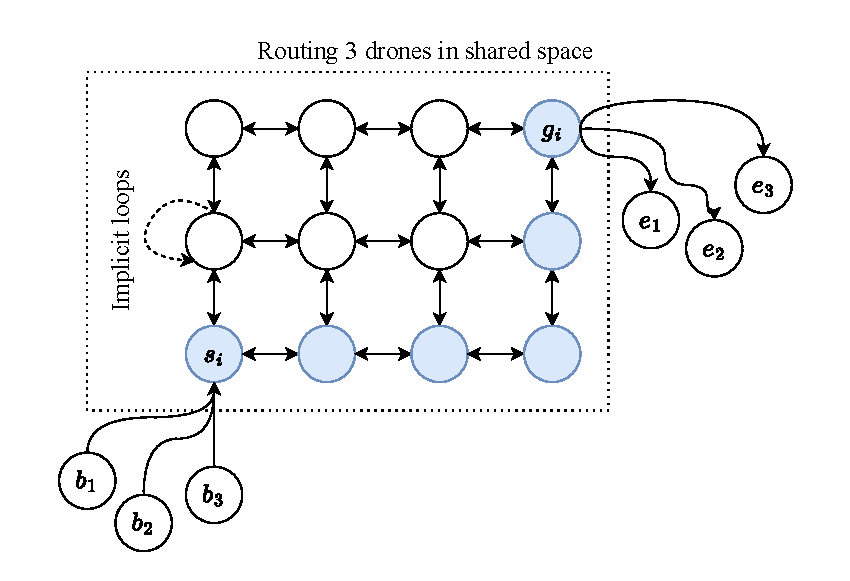
\includegraphics[width=0.8\textwidth]{img/worst_path.drawio.pdf}
    \caption{Worst case path.}
    \label{fig:worst_path}
\end{figure}



\subsection{Adaptability for 3D}

A notable difference from our method to others in MAPF is that our algorithm remains consistent across any grid dimension. That is, the algorithm for a 2D grid obtains solutions in the same way as for a 3D or 4D grid.

This fact becomes clear when we see that both our methods, the heuristic and the exact model, are based solely on the topology of the graph. There is no spatial dependency. When we increase the dimension to 3D, we are simply increasing the neighborhood of each node. In some sense, each vertex $v$ in 3D space will have two additional edges in its neighborhood (up and down).

Again, using the notation in Table \ref{tab:notation}, we can create a temporal graph $\mathcal{G}$ that naturally represents our problem in three dimensional space. The set of vertices $\mathcal{V} := (i,j,k,t)$ represents every possible position $(i,j,k)$ at any given time $t$ in our problem. Our definition is almost the same, the difference is we add one more index $k$ and consequently the possibility of the drone going up($k+1$) and down($k-1$). We achieve this by defining the set of outgoing edges for a vertex $v^* = (i^*,j^*,k^*,t^*)$ as $\mathcal{E}_{v^*} = \{ 
(i^*+1,j^*,k^*,t^*+1), 
(i^*,j^*+1,k^*,t^*+1), 
(i^*-1,j^*,k^*,t^*+1), 
(i^*,j^*-1,k^*,t^*+1), 
(i^*,j^*,k^*+1,t^*+1),
(i^*,j^*,k^*-1,t^*+1),
(i^*,j^*,k^*,t^*+1)
\}$.





\section{Hybrid Methodology}
\label{Hybrid_Methodology}

In this section, we propose a hybrid approach to solve the problem. Our hybrid methodology combines the strengths of both the heuristic approach presented in Section \ref{Heuristic} and the MILP model outlined in Section \ref{Mathematical_Model}. By leveraging the efficiency of the heuristic to quickly generate a feasible solution and then refining it using the exact model, we aim to achieve a balance between computational speed and solution optimality.

\subsection{Algorithm Overview}

We can outline the hybrid method sequentially. The methodology proceeds through the following steps:

\subsubsection{Heuristic Solution Generation}

The first step involves employing the heuristic algorithm to generate an initial feasible solution. The heuristic algorithm determines the time horizon $T_{\text{heuristic}}$ and computes paths for drones based on their initial positions and problem parameters.

\subsubsection{MILP Model Refinement}

Once the heuristic completes its execution, we utilize the time horizon $T_{\text{heuristic}}$ along with the initial drone positions and grid size parameters as input to the MILP model. Also, we modify the initial model variables to be the initial feasible point found by the heuristic, that is, the solver will already start the search in a local optimum point. The MILP model refines the solution within the time frame $T_{\text{heuristic}}$, ensuring optimality while maintaining computational efficiency.

\subsection{Advantages and Considerations}

The hybrid methodology offers several advantages:

\begin{itemize}
  \item \textbf{Computational Efficiency}: Leveraging the heuristic for initial solution generation reduces computational time compared to relying solely on the MILP model. Since we would have no warm start and would need to start with a guessed $T$, that in general would be high.
  \item \textbf{Global Optimality}: Refinement using the MILP model ensures the final solution achieves global optimality.
  \item \textbf{Flexibility and Adaptability}: Dynamic integration of the heuristic and MILP model allows for handling diverse problem instances and adapting to varying computational resources.
\end{itemize}

The main reason, that makes the hybrid method an useful one, is that we can skip the part where we need to determine $T$. Since, using just the MILP model we would need to test lots of $T_s$ to determine which one    to use, for each $T$ we would need to solve an other instance of the problem and when finding a infeasible solution return $(T+1)$. A simple algorithm would be: \mintinline{cpp}{while(T--){ if(is_infeasible(T) return T+1;}}, for a high guess of T, that is, in the worst case we would solve $\mathcal{O}(T)$ instances of the mathematical model, which is expensive. When we get the $T$ from the heuristic we guarantee the MILP solver search to be in a plausible $T$ close to the optimal.

However, potential trade-offs include computational complexity and the need for careful validation and testing. The success of the hybrid methodology relies on the synergy between the heuristic and MILP model components.  Although in this work we do not experiment the hybrid method, in Section \ref{sec:transition} we show that using $T_{\text{heuristic}}$ as a guess $T$ for the exact model is reasonable, since $T$ is linear in the number of drones.



